\section{Accuracy of modelfitting}

\subsection{Ranges and resolutions}

One of the major problems faced throughout the development of the modelfitting algorithm was with the selection of ranges and resolutions.
In Listing \ref{leastsquarescode} there is a mention of four variables - $range_\theta$, $range_\alpha$, $resolution_\theta$ and $resolution_\alpha$.
These variables control the size and resolution of the parameter space that is searched during the modelfitting.
Care must be taken when adjusting these variables as they control both the accuracy of the results and the execution time of the algorithm.

Some of the problems encountered when selecting values for the variables are given below.

\begin{figure}[p]
	\centering
	\subfloat[Left thigh energy]{\label{Alpha:GoodLeftThigh}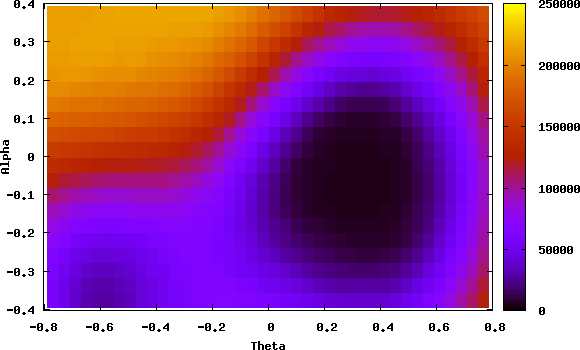
\includegraphics[width=6.2cm]{problems/good-leftthigh.png}}
	\qquad
	\subfloat[Right thigh energy]{\label{Alpha:GoodRightThigh}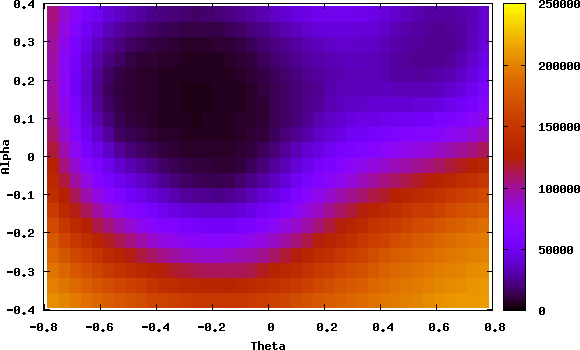
\includegraphics[width=6.2cm]{problems/good-rightthigh.png}}
	\\
	\subfloat[Left lower leg energy]{\label{Alpha:GoodLeftLower}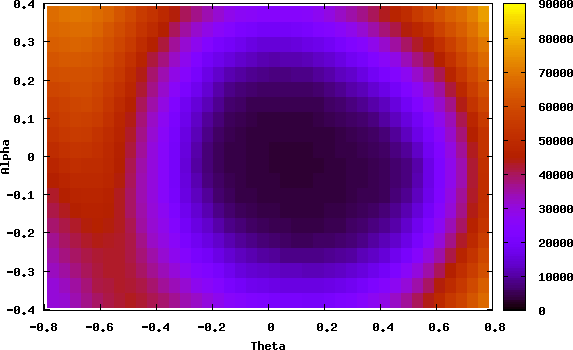
\includegraphics[width=6.2cm]{problems/good-leftlower.png}}
	\qquad
	\subfloat[Right lower leg energy]{\label{Alpha:GoodRightLower}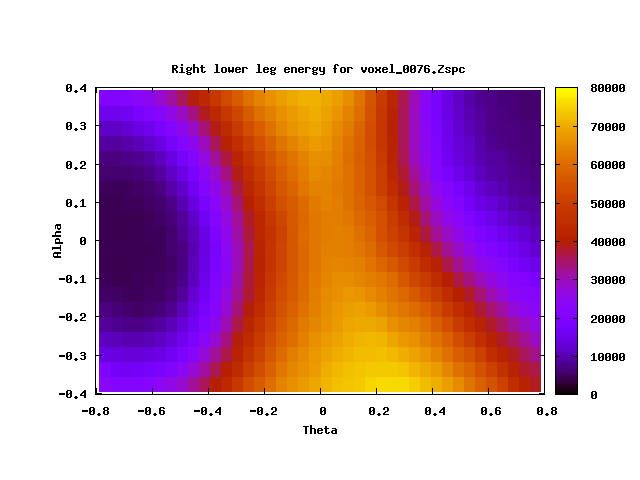
\includegraphics[width=6.2cm]{problems/good-rightlower.png}}
	\\
	\subfloat[Model and voxel data]{\label{Alpha:Good3D}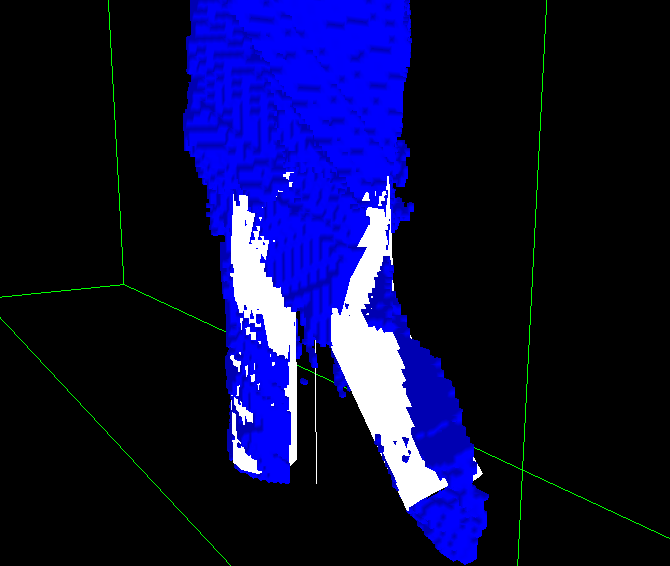
\includegraphics[width=6.2cm]{problems/good-3d.png}}
	\qquad
	\subfloat[Model]{\label{Alpha:GoodModel}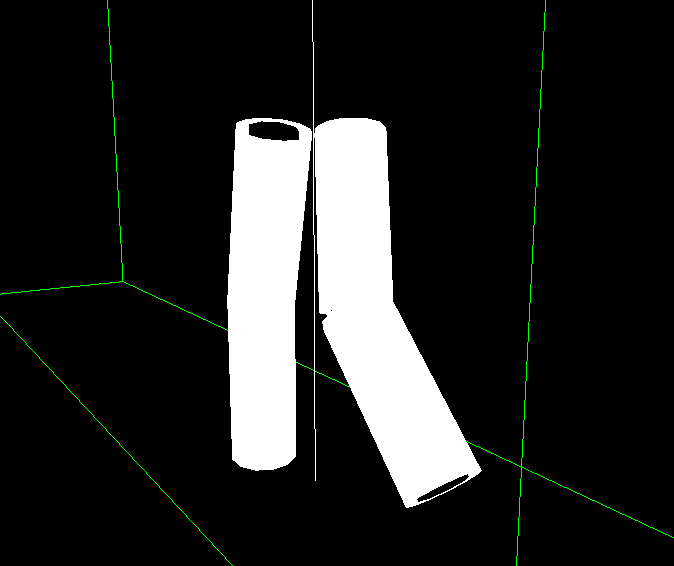
\includegraphics[width=6.2cm]{problems/good-model.png}}
	
	\caption{Frame 76, a good fitting of the model to the data.
		Notice in \ref{Alpha:GoodRightThigh} how there is a local minimum developing in the upper-right corner.
		Remember that \ref{Alpha:GoodRightThigh} and \ref{Alpha:GoodRightLower} are slices through a four-dimensional space,
		and as such there may be minima elsewhere that are not shown.}
	\label{AlphaGood}
\end{figure}

\begin{figure}[p]
	\centering
	\subfloat[Left thigh energy]{\label{Alpha:BadLeftThigh}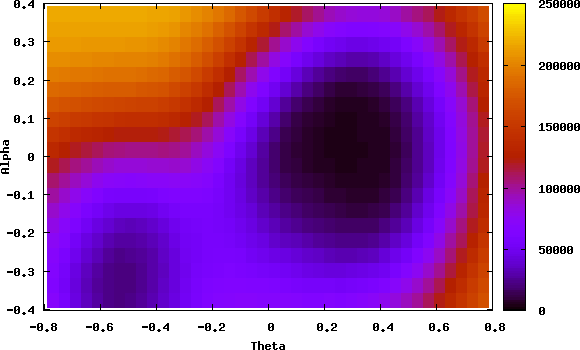
\includegraphics[width=6.2cm]{problems/badalpha-leftthigh.png}}
	\qquad
	\subfloat[Right thigh energy]{\label{Alpha:BadRightThigh}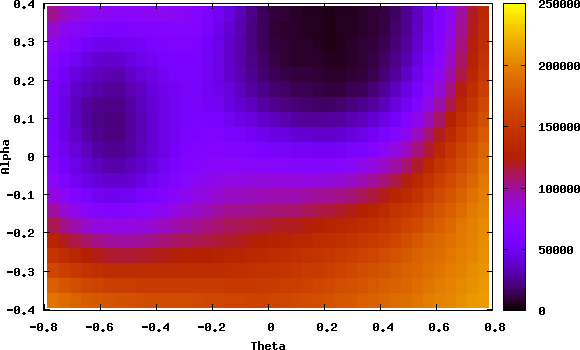
\includegraphics[width=6.2cm]{problems/badalpha-rightthigh.png}}
	\\
	\subfloat[Left lower leg energy]{\label{Alpha:BadLeftLower}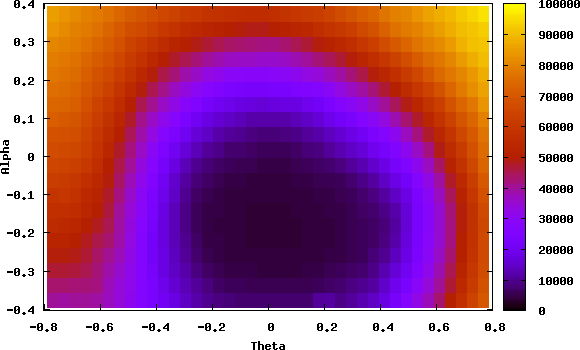
\includegraphics[width=6.2cm]{problems/badalpha-leftlower.png}}
	\qquad
	\subfloat[Right lower leg energy]{\label{Alpha:BadRightLower}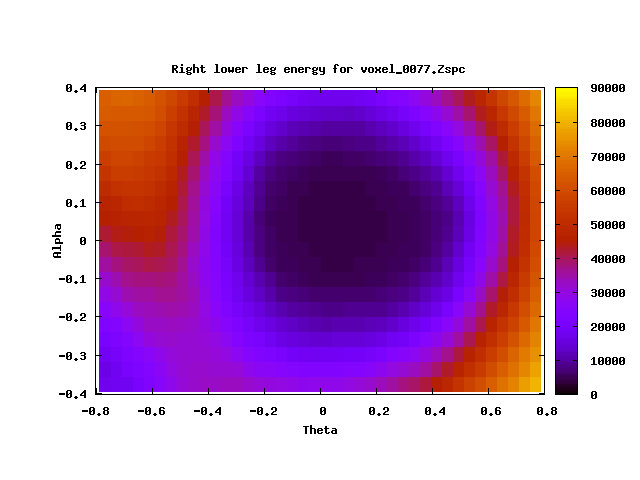
\includegraphics[width=6.2cm]{problems/badalpha-rightlower.png}}
	\\
	\subfloat[Model and voxel data]{\label{Alpha:Bad3D}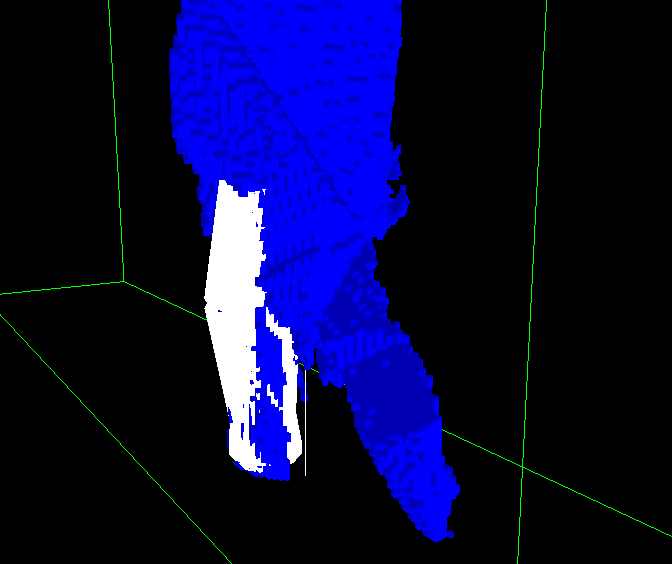
\includegraphics[width=6.2cm]{problems/badalpha-3d.png}}
	\qquad
	\subfloat[Model]{\label{Alpha:BadModel}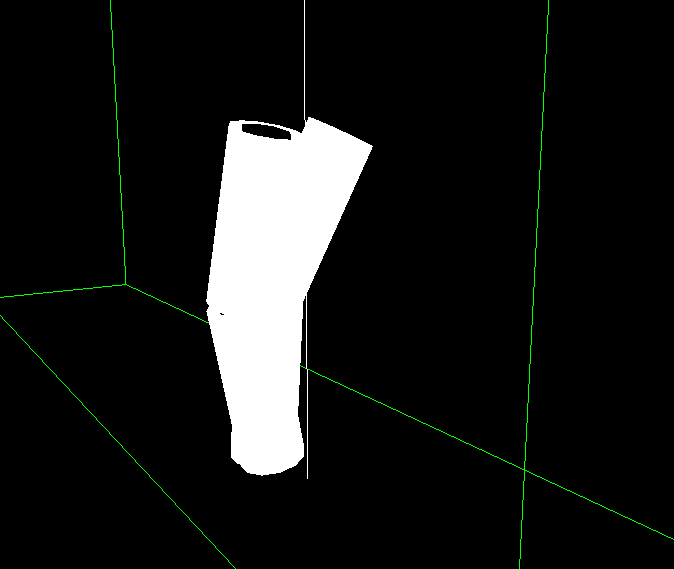
\includegraphics[width=6.2cm]{problems/badalpha-model.png}}
	
	\caption{Frame 77, an erroneous fitting of the model to the data.
		The local minimum in \ref{Alpha:GoodRightThigh} on the previous page must have had a much lower energy with $(\alpha_2, \theta_2) = (0, 0)$ (lower leg energy).
		In this frame the energy at that point became even lower - lower than that of the correct point - and became the global minimum.}
	\label{AlphaBad}
\end{figure}

\begin{enumerate}
	\item \textbf{Erroneous minima}.
		Originally we had set $range_\alpha = \left[ -\frac{\pi}{8}, +\frac{\pi}{8}\right]$.
		This range turned out to be far too big, and as such would lead to erroneous minima being found.
		The problem tended to occur when the two thighs were close together - one of the thighs would assume
		a large alpha value and swing towards the subject's other leg.
		The two leg models would then intersect as they matched the same leg in the data.
		
		Figures \ref{AlphaGood} and \ref{AlphaBad} demonstrate this problem.
		They are of subsequent frames in sample 81 - the first frame matches the right leg correctly
		but the second frame is incorrect.
		The right thigh has an alpha value that is strongly positive, and this leads to it matching most of the left leg instead.
		
		To understand why this has happened we need to remember that the parameter space is four-dimensional, and each of the energy plots
		shown are only slices with two of the parameters held constant.
		Therefore much of the parameter space is not shown in the plots.
		Figure \ref{Alpha:GoodRightThigh} shows a small low energy region near the top, in a similar location to the larger low energy region in Figure \ref{Alpha:BadRightThigh}.
		The energy of this region in the first plot is not nearly as low as the other, correct, minimum, so we may wonder why it has grown so dramatically between frames.
		The answer is that Figure \ref{Alpha:GoodRightThigh} is a slice at the minimum in Figure \ref{Alpha:GoodRightLower} - if we moved it so the slice
		were instead taken at the minimum from Figure \ref{Alpha:BadRightLower} we would likely see a much stronger low energy region.
		
		This was a major problem, and a number of approaches were taken to attempt to solve it.
		The first was to smooth the data - using the results of the previous frames to apply a penalty to parameters that were too far away from the expected position.
		However this seemed more like a remedy to the result of the problem (wrong minima being chosen) rather than the cause of it (bad alpha range).
		Also it was feared that any kind of smoothing of the data might destroy valuable gait information.
		
		Instead it was decided to take the simpler solution - limiting the range of possible alpha values.
		A strong distinction was noted between the typical alpha values of correct and incorrect frames - the correct frames all took on
		values within the range $\left[ -\frac{\pi}{32}, +\frac{\pi}{32}\right]$, and the others outside.
		$range_\alpha$ was therefore set to $\left[ -\frac{\pi}{32}, +\frac{\pi}{32}\right]$.
	
	\item \textbf{Oversampling}.
		There is a limit to the maximum resolution at which it is sensible to sample the parameter space.
		The size of the voxels in the data is $1\text{cm}^3$.
		Comparing the fitting of two orientations of the model that differ by less than $1\text{cm}^3$ is meaningless,
		as the coordinates of every distance lookup performed are clamped to integer values (not doing so would break
		the lookup cache from section TODO).
		
		Sampling at these high resolutions could not be considered before multi-resolution sampling (TODO) was implemented
		as the execution time would have been prohibitive.
		With the introduction of multi-resolution sampling however some high-resolution fittings were tested, and as expected
		the noise resulting from the discrete nature of the data led to errors in the DFT and a lower classification rate.
		
		The ideal resolutions were discovered to be $resolution_\theta = 41$ and $resolution_\alpha = 11$ - meaning the
		parameter space is 41x41x11x11 (odd numbers were chosen to ensure there is one sample taken at $(0, 0, 0, 0)$).
\end{enumerate}


\subsection{Quantitative error analysis}

Comparison with manually fit data.
Show some graphs of theta over time.